% !TEX root = ../report.tex
\chapter{Ergebnisse}
\begin{Spacing}{\mylinespace}

Mit diesem Projekt ist es gelungen, die Simulation einer Strömung nachzubilden. Es kann in direkt Einfluss auf die Strömung genommen werden, indem z.B. ein kleiner Berg aus Sand gebaut wird.

Durch die Nutzung der GPU, zur Berechnung und Darstellung, kann eine hohe Anzahl von Partikeln angezeigt werden. Die Physikberechnung im Hintergrund trägt dazu bei das sich die Partikel mit der Strömung realistisch durch die Umgebung bewegen. Wie in Abbildung \ref{fig:Results} zu sehen ist, wird die \textit{Sandhöhe} farblich dargestellt. Die Strömung wird durch weiße Partikel Simuliert. Die Anpassung der Bilder des Projektors sowie der Tiefenkamera sind mechanisch ausreichend ausgeführt. Das Umströmen eingebrachter Fremdkörper wie z.B. eines Modelhauses oder LKWs bewirkt, wie gewünscht, eine Beeinflussung des Partikelstromes. 

\begin{figure}[h!]
	\vspace*{30px}
	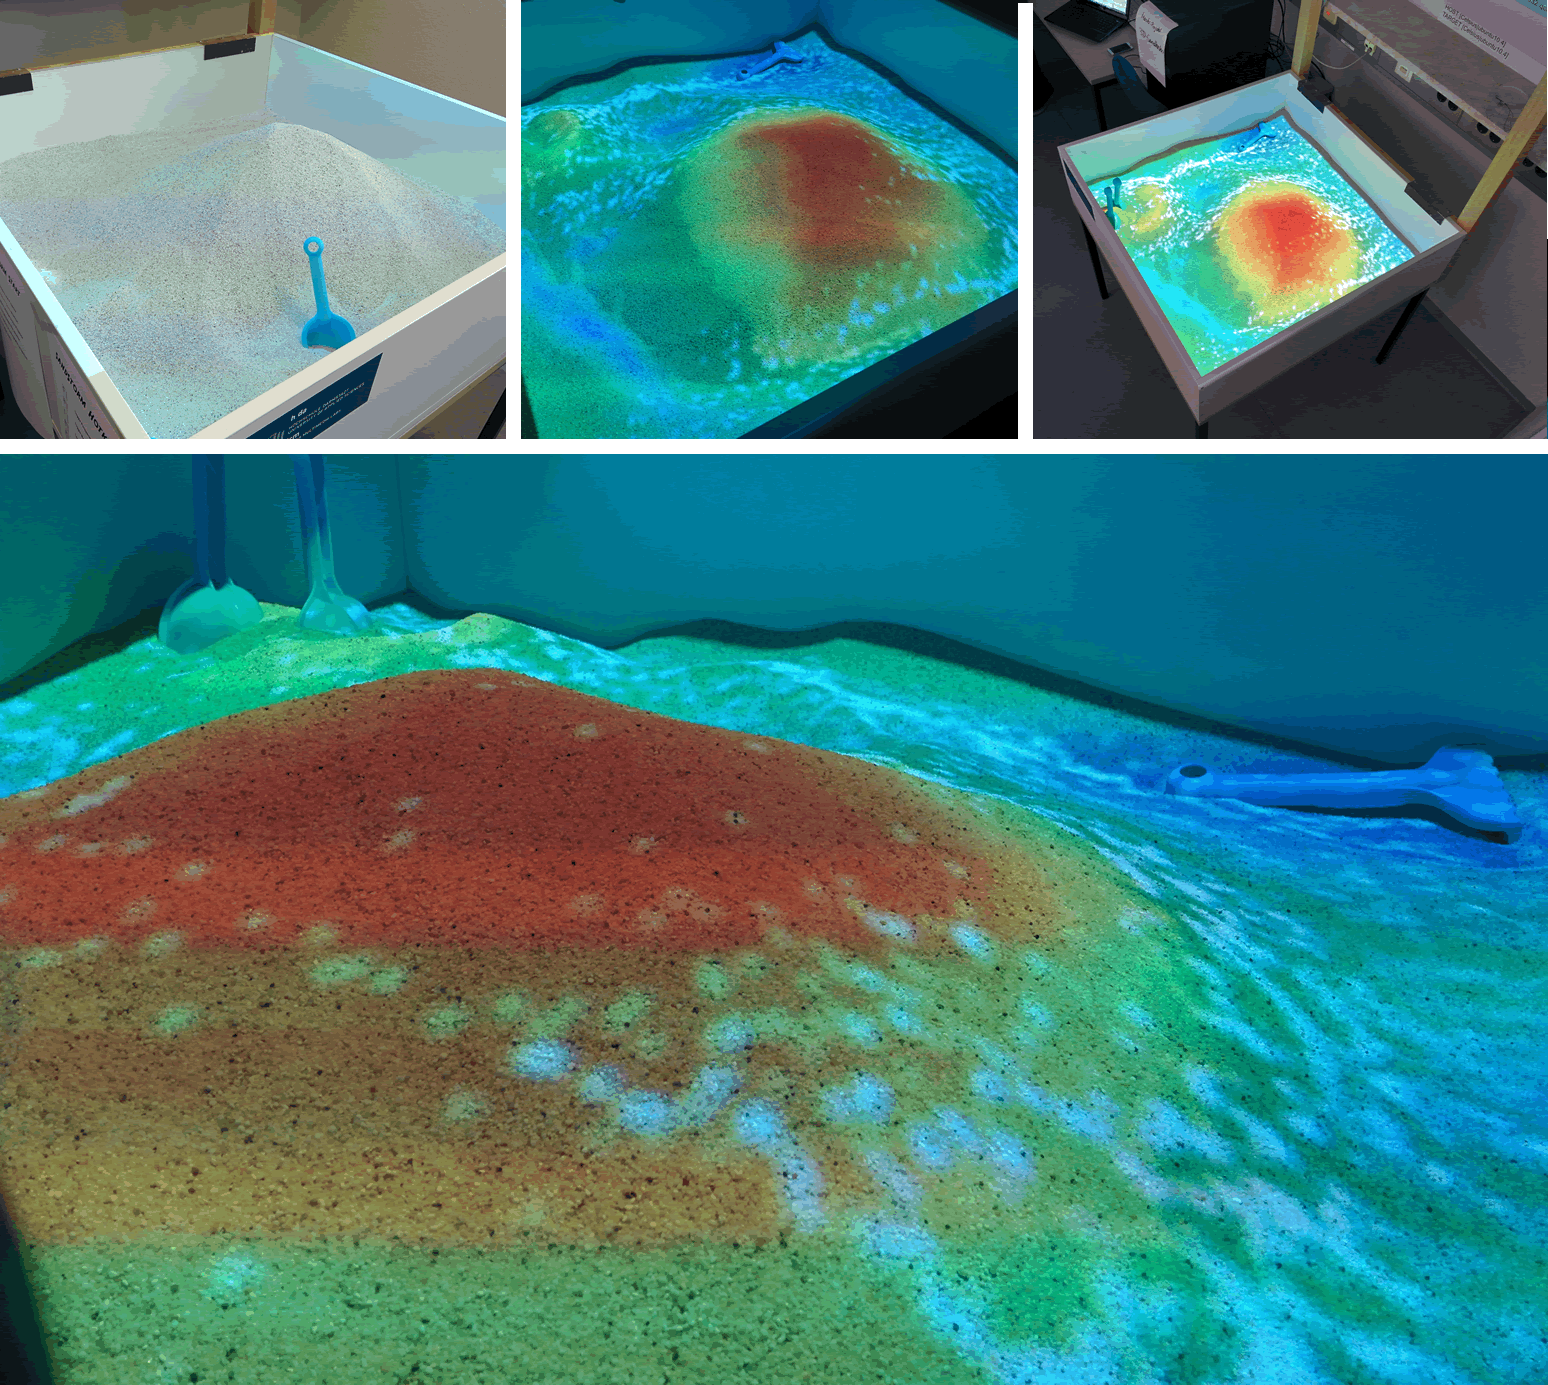
\includegraphics[width=\textwidth]{graphics/results.png}	
	\caption{Sandstorm Projekt in Betrieb}
	\label{fig:Results}
\end{figure}

\end{Spacing}
\newpage
\clearpage
%% End Of Doc